\documentclass{standalone}
\usepackage{pgfplots}

\begin{document}
	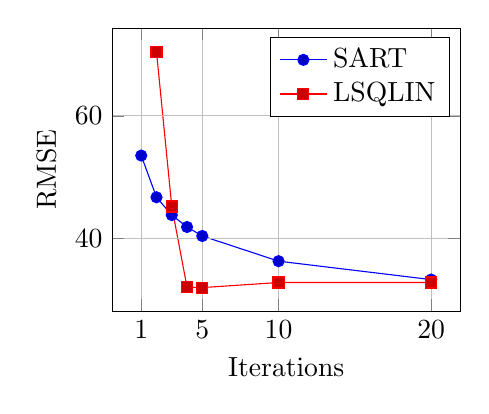
\begin{tikzpicture}
		
		\begin{axis}[	legend pos = north east, 
						legend cell align = left,
						xtick = {1, 5, 10, 20},
						ylabel = {RMSE},
						xlabel = {Iterations},
						ylabel near ticks,
						grid = major,
						axis on top = true,
						width = 6 cm]
		
			\addplot coordinates {
				(1, 53.517116)
				(2, 46.6983)
				(3, 43.7923)
				(4, 41.8413)
				(5, 40.3709)
				(10, 36.2524)
				(20, 33.2420)
			};
			\addlegendentry{SART};
			
			\addplot coordinates {
				(2, 70.477447)
				(3, 45.188843)
				(4, 32.001308)
				(5, 31.934515)
				(10, 32.764468)
				(20, 32.766828)
			};
			\addlegendentry{LSQLIN};
			
			 
		\end{axis}
		
	\end{tikzpicture}
\end{document}